\FChapter{Chapter Eighteen}{18}

\Lettrine{M}{erry} \textsc{days} were these at Thornfield Hall; and busy days too: how
different from the first three months of stillness, monotony, and
solitude I had passed beneath its roof! All sad feelings seemed now
driven from the house, all gloomy associations forgotten: there was life
everywhere, movement all day long. You could not now traverse the
gallery, once so hushed, nor enter the front chambers, once so
tenantless, without encountering a smart lady's-maid or a dandy valet.

The kitchen, the butler's pantry, the servants' hall, the entrance hall,
were equally alive; and the saloons were only left void and still when
the blue sky and halcyon sunshine of the genial spring weather called
their occupants out into the grounds. Even when that weather was
broken, and continuous rain set in for some days, no damp seemed cast
over enjoyment: indoor amusements only became more lively and varied, in
consequence of the stop put to outdoor gaiety.

I wondered what they were going to do the first evening a change of
entertainment was proposed: they spoke of \enquote{playing charades,}
but in my ignorance I did not understand the term. The servants were
called in, the dining-room tables wheeled away, the lights otherwise
disposed, the chairs placed in a semicircle opposite the arch. While
\Mr{} Rochester and the other gentlemen directed these alterations, the
ladies were running up and down stairs ringing for their maids. \Mrs{}
Fairfax was summoned to give information respecting the resources of the
house in shawls, dresses, draperies of any kind; and certain wardrobes
of the third storey were ransacked, and their contents, in the shape of
brocaded and hooped petticoats, satin sacques, black modes, lace
lappets, \etc, were brought down in armfuls by the abigails; then a
selection was made, and such things as were chosen were carried to the
boudoir within the drawing-room.

Meantime, \Mr{} Rochester had again summoned the ladies round him, and was
selecting certain of their number to be of his party. \enquote{Miss
	Ingram is mine, of course,} said he: afterwards he named the two Misses
Eshton, and \Mrs{} Dent. He looked at me: I happened to be near him, as I
had been fastening the clasp of \Mrs{} Dent's bracelet, which had got
loose.

\enquote{Will you play?} he asked. I shook my head. He did not insist,
which I rather feared he would have done; he allowed me to return
quietly to my usual seat.

He and his aids now withdrew behind the curtain: the other party, which
was headed by Colonel Dent, sat down on the crescent of chairs. One of
the gentlemen, \Mr{} Eshton, observing me, seemed to propose that I should
be asked to join them; but Lady Ingram instantly negatived the notion.

\enquote{No,} I heard her say: \enquote{she looks too stupid for any
	game of the sort.}

Ere long a bell tinkled, and the curtain drew up. Within the arch, the
bulky figure of Sir George Lynn, whom \Mr{} Rochester had likewise chosen,
was seen enveloped in a white sheet: before him, on a table, lay open a
large book; and at his side stood Amy Eshton, draped in \Mr{} Rochester's
cloak, and holding a book in her hand. Somebody, unseen, rang the bell
merrily; then Adèle (who had insisted on being one of her guardian's
party), bounded forward, scattering round her the contents of a basket
of flowers she carried on her arm. Then appeared the magnificent figure
of Miss Ingram, clad in white, a long veil on her head, and a wreath of
roses round her brow; by her side walked \Mr{} Rochester, and together
they drew near the table. They knelt; while \Mrs{} Dent and Louisa
Eshton, dressed also in white, took up their stations behind them. A
ceremony followed, in dumb show, in which it was easy to recognise the
pantomime of a marriage. At its termination, Colonel Dent and his party
consulted in whispers for two minutes, then the Colonel called out---

\enquote{Bride!} \Mr{} Rochester bowed, and the curtain fell.

A considerable interval elapsed before it again rose. Its second rising
displayed a more elaborately prepared scene than the last. The
drawing-room, as I have before observed, was raised two steps above the
dining-room, and on the top of the upper step, placed a yard or two back
within the room, appeared a large marble basin---which I recognised as
an ornament of the conservatory---where it usually stood, surrounded by
exotics, and tenanted by gold fish---and whence it must have been
transported with some trouble, on account of its size and weight.

Seated on the carpet, by the side of this basin, was seen \Mr{} Rochester,
costumed in shawls, with a turban on his head. His dark eyes and
swarthy skin and Paynim features suited the costume exactly: he looked
the very model of an Eastern emir, an agent or a victim of the
bowstring. Presently advanced into view Miss Ingram. She, too, was
attired in oriental fashion: a crimson scarf tied sash-like round the
waist: an embroidered handkerchief knotted about her temples; her
beautifully-moulded arms bare, one of them upraised in the act of
supporting a pitcher, poised gracefully on her head. Both her cast of
form and feature, her complexion and her general air, suggested the idea
of some Israelitish princess of the patriarchal days; and such was
doubtless the character she intended to represent.

She approached the basin, and bent over it as if to fill her pitcher;
she again lifted it to her head. The personage on the well-brink now
seemed to accost her; to make some request:---\enquote{She hasted, let
	down her pitcher on her hand, and gave him to drink.} From the bosom of
his robe he then produced a casket, opened it and showed magnificent
bracelets and earrings; she acted astonishment and admiration; kneeling,
he laid the treasure at her feet; incredulity and delight were expressed
by her looks and gestures; the stranger fastened the bracelets on her
arms and the rings in her ears. It was Eliezer and Rebecca: the camels
only were wanting.

The divining party again laid their heads together: apparently they
could not agree about the word or syllable the scene illustrated.
Colonel Dent, their spokesman, demanded \enquote{the tableau of the
	whole;} whereupon the curtain again descended.

On its third rising only a portion of the drawing-room was disclosed;
the rest being concealed by a screen, hung with some sort of dark and
coarse drapery. The marble basin was removed; in its place, stood a
deal table and a kitchen chair: these objects were visible by a very dim
light proceeding from a horn lantern, the wax candles being all
extinguished.

Amidst this sordid scene, sat a man with his clenched hands resting on
his knees, and his eyes bent on the ground. I knew \Mr{} Rochester;
though the begrimed face, the disordered dress (his coat hanging loose
from one arm, as if it had been almost torn from his back in a scuffle),
the desperate and scowling countenance, the rough, bristling hair might
well have disguised him. As he moved, a chain clanked; to his wrists
were attached fetters.

\enquote{Bridewell!} exclaimed Colonel Dent, and the charade was solved.

A sufficient interval having elapsed for the performers to resume their
ordinary costume, they re-entered the dining-room. \Mr{} Rochester led in
Miss Ingram; she was complimenting him on his acting.

\enquote{Do you know,} said she, \enquote{that, of the three characters,
	I liked you in the last best? Oh, had you but lived a few years
	earlier, what a gallant gentleman-highwayman you would have made!}

\enquote{Is all the soot washed from my face?} he asked, turning it
towards her.

\enquote{Alas! yes: the more's the pity! Nothing could be more becoming
	to your complexion than that ruffian's rouge.}

\enquote{You would like a hero of the road then?}

\enquote{An English hero of the road would be the next best thing to an
	Italian bandit; and that could only be surpassed by a Levantine pirate.}

\enquote{Well, whatever I am, remember you are my wife; we were married
	an hour since, in the presence of all these witnesses.} She giggled,
and her colour rose.

\enquote{Now, Dent,} continued \Mr{} Rochester, \enquote{it is your
	turn.} And as the other party withdrew, he and his band took the
vacated seats. Miss Ingram placed herself at her leader's right hand;
the other diviners filled the chairs on each side of him and her. I did
not now watch the actors; I no longer waited with interest for the
curtain to rise; my attention was absorbed by the spectators; my eyes,
erewhile fixed on the arch, were now irresistibly attracted to the
semicircle of chairs. What charade Colonel Dent and his party played,
what word they chose, how they acquitted themselves, I no longer
remember; but I still see the consultation which followed each scene: I
see \Mr{} Rochester turn to Miss Ingram, and Miss Ingram to him; I see her
incline her head towards him, till the jetty curls almost touch his
shoulder and wave against his cheek; I hear their mutual whisperings; I
recall their interchanged glances; and something even of the feeling
roused by the spectacle returns in memory at this moment.

I have told you, reader, that I had learnt to love \Mr{} Rochester: I
could not unlove him now, merely because I found that he had ceased to
notice me---because I might pass hours in his presence, and he would
never once turn his eyes in my direction---because I saw all his
attentions appropriated by a great lady, who scorned to touch me with
the hem of her robes as she passed; who, if ever her dark and imperious
eye fell on me by chance, would withdraw it instantly as from an object
too mean to merit observation. I could not unlove him, because I felt
sure he would soon marry this very lady---because I read daily in her a
proud security in his intentions respecting her---because I witnessed
hourly in him a style of courtship which, if careless and choosing
rather to be sought than to seek, was yet, in its very carelessness,
captivating, and in its very pride, irresistible.

There was nothing to cool or banish love in these circumstances, though
much to create despair. Much too, you will think, reader, to engender
jealousy: if a woman, in my position, could presume to be jealous of a
woman in Miss Ingram's. But I was not jealous: or very rarely;---the
nature of the pain I suffered could not be explained by that word. Miss
Ingram was a mark beneath jealousy: she was too inferior to excite the
feeling. Pardon the seeming paradox; I mean what I say. She was very
showy, but she was not genuine: she had a fine person, many brilliant
attainments; but her mind was poor, her heart barren by nature: nothing
bloomed spontaneously on that soil; no unforced natural fruit delighted
by its freshness. She was not good; she was not original: she used to
repeat sounding phrases from books: she never offered, nor had, an
opinion of her own. She advocated a high tone of sentiment; but she did
not know the sensations of sympathy and pity; tenderness and truth were
not in her. Too often she betrayed this, by the undue vent she gave to
a spiteful antipathy she had conceived against little Adèle: pushing her
away with some contumelious epithet if she happened to approach her;
sometimes ordering her from the room, and always treating her with
coldness and acrimony. Other eyes besides mine watched these
manifestations of character---watched them closely, keenly, shrewdly.
Yes; the future bridegroom, \Mr{} Rochester himself, exercised over his
intended a ceaseless surveillance; and it was from this sagacity---this
guardedness of his---this perfect, clear consciousness of his fair one's
defects---this obvious absence of passion in his sentiments towards her,
that my ever-torturing pain arose.

I saw he was going to marry her, for family, perhaps political reasons,
because her rank and connections suited him; I felt he had not given her
his love, and that her qualifications were ill adapted to win from him
that treasure. This was the point---this was where the nerve was
touched and teased---this was where the fever was sustained and fed:
\emph{she could not charm him}.

If she had managed the victory at once, and he had yielded and sincerely
laid his heart at her feet, I should have covered my face, turned to the
wall, and (figuratively) have died to them. If Miss Ingram had been a
good and noble woman, endowed with force, fervour, kindness, sense, I
should have had one vital struggle with two tigers---jealousy and
despair: then, my heart torn out and devoured, I should have admired
her---acknowledged her excellence, and been quiet for the rest of my
days: and the more absolute her superiority, the deeper would have been
my admiration---the more truly tranquil my quiescence. But as matters
really stood, to watch Miss Ingram's efforts at fascinating \Mr{}
Rochester, to witness their repeated failure---herself unconscious that
they did fail; vainly fancying that each shaft launched hit the mark,
and infatuatedly pluming herself on success, when her pride and
self-complacency repelled further and further what she wished to
allure---to witness \emph{this}, was to be at once under ceaseless
excitation and ruthless restraint.

Because, when she failed, I saw how she might have succeeded. Arrows
that continually glanced off from \Mr{} Rochester's breast and fell
harmless at his feet, might, I knew, if shot by a surer hand, have
quivered keen in his proud heart---have called love into his stern eye,
and softness into his sardonic face; or, better still, without weapons a
silent conquest might have been won.

\enquote{Why can she not influence him more, when she is privileged to
	draw so near to him?} I asked myself. \enquote{Surely she cannot truly
	like him, or not like him with true affection! If she did, she need not
	coin her smiles so lavishly, flash her glances so unremittingly,
	manufacture airs so elaborate, graces so multitudinous. It seems to me
	that she might, by merely sitting quietly at his side, saying little and
	looking less, get nigher his heart. I have seen in his face a far
	different expression from that which hardens it now while she is so
	vivaciously accosting him; but then it came of itself: it was not
	elicited by meretricious arts and calculated manoeuvres; and one had but
	to accept it---to answer what he asked without pretension, to address
	him when needful without grimace---and it increased and grew kinder and
	more genial, and warmed one like a fostering sunbeam. How will she
	manage to please him when they are married? I do not think she will
	manage it; and yet it might be managed; and his wife might, I verily
	believe, be the very happiest woman the sun shines on.}

I have not yet said anything condemnatory of \Mr{} Rochester's project of
marrying for interest and connections. It surprised me when I first
discovered that such was his intention: I had thought him a man unlikely
to be influenced by motives so commonplace in his choice of a wife; but
the longer I considered the position, education, \etc, of the parties,
the less I felt justified in judging and blaming either him or Miss
Ingram for acting in conformity to ideas and principles instilled into
them, doubtless, from their childhood. All their class held these
principles: I supposed, then, they had reasons for holding them such as
I could not fathom. It seemed to me that, were I a gentleman like him,
I would take to my bosom only such a wife as I could love; but the very
obviousness of the advantages to the husband's own happiness offered by
this plan convinced me that there must be arguments against its general
adoption of which I was quite ignorant: otherwise I felt sure all the
world would act as I wished to act.

But in other points, as well as this, I was growing very lenient to my
master: I was forgetting all his faults, for which I had once kept a
sharp look-out. It had formerly been my endeavour to study all sides of
his character: to take the bad with the good; and from the just weighing
of both, to form an equitable judgment. Now I saw no bad. The sarcasm
that had repelled, the harshness that had startled me once, were only
like keen condiments in a choice dish: their presence was pungent, but
their absence would be felt as comparatively insipid. And as for the
vague something---was it a sinister or a sorrowful, a designing or a
desponding expression?---that opened upon a careful observer, now and
then, in his eye, and closed again before one could fathom the strange
depth partially disclosed; that something which used to make me fear and
shrink, as if I had been wandering amongst volcanic-looking hills, and
had suddenly felt the ground quiver and seen it gape: that something, I,
at intervals, beheld still; and with throbbing heart, but not with
palsied nerves. Instead of wishing to shun, I longed only to dare---to
divine it; and I thought Miss Ingram happy, because one day she might
look into the abyss at her leisure, explore its secrets and analyse
their nature.

Meantime, while I thought only of my master and his future bride---saw
only them, heard only their discourse, and considered only their
movements of importance---the rest of the party were occupied with their
own separate interests and pleasures. The Ladies Lynn and Ingram
continued to consort in solemn conferences, where they nodded their two
turbans at each other, and held up their four hands in confronting
gestures of surprise, or mystery, or horror, according to the theme on
which their gossip ran, like a pair of magnified puppets. Mild \Mrs{}
Dent talked with good-natured \Mrs{} Eshton; and the two sometimes
bestowed a courteous word or smile on me. Sir George Lynn, Colonel
Dent, and \Mr{} Eshton discussed politics, or county affairs, or justice
business. Lord Ingram flirted with Amy Eshton; Louisa played and sang
to and with one of the Messrs. Lynn; and Mary Ingram listened languidly
to the gallant speeches of the other. Sometimes all, as with one
consent, suspended their by-play to observe and listen to the principal
actors: for, after all, \Mr{} Rochester and---because closely connected
with him---Miss Ingram were the life and soul of the party. If he was
absent from the room an hour, a perceptible dulness seemed to steal over
the spirits of his guests; and his re-entrance was sure to give a fresh
impulse to the vivacity of conversation.

The want of his animating influence appeared to be peculiarly felt one
day that he had been summoned to Millcote on business, and was not
likely to return till late. The afternoon was wet: a walk the party had
proposed to take to see a gipsy camp, lately pitched on a common beyond
Hay, was consequently deferred. Some of the gentlemen were gone to the
stables: the younger ones, together with the younger ladies, were
playing billiards in the billiard-room. The dowagers Ingram and Lynn
sought solace in a quiet game at cards. Blanche Ingram, after having
repelled, by supercilious taciturnity, some efforts of \Mrs{} Dent and
\Mrs{} Eshton to draw her into conversation, had first murmured over some
sentimental tunes and airs on the piano, and then, having fetched a
novel from the library, had flung herself in haughty listlessness on a
sofa, and prepared to beguile, by the spell of fiction, the tedious
hours of absence. The room and the house were silent: only now and then
the merriment of the billiard-players was heard from above.

It was verging on dusk, and the clock had already given warning of the
hour to dress for dinner, when little Adèle, who knelt by me in the
drawing-room window-seat, suddenly exclaimed---

\foreignquote{french}{Voilà, Monsieur Rochester, qui revient!}\footnote{
	\enquote{Here, \Mr{} Rochester, coming home!}}

I turned, and Miss Ingram darted forwards from her sofa: the others,
too, looked up from their several occupations; for at the same time a
crunching of wheels and a splashing tramp of horse-hoofs became audible
on the wet gravel. A post-chaise was approaching.

\enquote{What can possess him to come home in that style?} said Miss
Ingram. \enquote{He rode Mesrour (the black horse), did he not, when he
	went out? and Pilot was with him:---what has he done with the animals?}

As she said this, she approached her tall person and ample garments so
near the window, that I was obliged to bend back almost to the breaking
of my spine: in her eagerness she did not observe me at first, but when
she did, she curled her lip and moved to another casement. The
post-chaise stopped; the driver rang the door-bell, and a gentleman
alighted attired in travelling garb; but it was not \Mr{} Rochester; it
was a tall, fashionable-looking man, a stranger.

\enquote{How provoking!} exclaimed Miss Ingram: \enquote{you tiresome
	monkey!} (apostrophising Adèle), \enquote{who perched you up in the
	window to give false intelligence?} and she cast on me an angry glance,
as if I were in fault.

Some parleying was audible in the hall, and soon the new-comer entered.
He bowed to Lady Ingram, as deeming her the eldest lady present.

\enquote{It appears I come at an inopportune time, madam,} said he,
\enquote{when my friend, \Mr{} Rochester, is from home; but I arrive from
	a very long journey, and I think I may presume so far on old and
	intimate acquaintance as to instal myself here till he returns.}

His manner was polite; his accent, in speaking, struck me as being
somewhat unusual,---not precisely foreign, but still not altogether
English: his age might be about \Mr{} Rochester's,---between thirty and
forty; his complexion was singularly sallow: otherwise he was a
fine-looking man, at first sight especially. On closer examination, you
detected something in his face that displeased, or rather that failed to
please. His features were regular, but too relaxed: his eye was large
and well cut, but the life looking out of it was a tame, vacant
life---at least so I thought.

The sound of the dressing-bell dispersed the party. It was not till
after dinner that I saw him again: he then seemed quite at his ease.
But I liked his physiognomy even less than before: it struck me as being
at the same time unsettled and inanimate. His eye wandered, and had no
meaning in its wandering: this gave him an odd look, such as I never
remembered to have seen. For a handsome and not an unamiable-looking
man, he repelled me exceedingly: there was no power in that
smooth-skinned face of a full oval shape: no firmness in that aquiline
nose and small cherry mouth; there was no thought on the low, even
forehead; no command in that blank, brown eye.

As I sat in my usual nook, and looked at him with the light of the
girandoles on the mantelpiece beaming full over him---for he occupied an
arm-chair drawn close to the fire, and kept shrinking still nearer, as
if he were cold, I compared him with \Mr{} Rochester. I think (with
deference be it spoken) the contrast could not be much greater between a
sleek gander and a fierce falcon: between a meek sheep and the
rough-coated keen-eyed dog, its guardian.

He had spoken of \Mr{} Rochester as an old friend. A curious friendship
theirs must have been: a pointed illustration, indeed, of the old adage
that \enquote{extremes meet.}

Two or three of the gentlemen sat near him, and I caught at times scraps
of their conversation across the room. At first I could not make much
sense of what I heard; for the discourse of Louisa Eshton and Mary
Ingram, who sat nearer to me, confused the fragmentary sentences that
reached me at intervals. These last were discussing the stranger; they
both called him \enquote{a beautiful man.} Louisa said he was
\enquote{a love of a creature,} and she \enquote{adored him;} and Mary
instanced his \enquote{pretty little mouth, and nice nose,} as her ideal
of the charming.

\enquote{And what a sweet-tempered forehead he has!} cried
Louisa,---\enquote{so smooth---none of those frowning irregularities I
	dislike so much; and such a placid eye and smile!}

And then, to my great relief, \Mr{} Henry Lynn summoned them to the other
side of the room, to settle some point about the deferred excursion to
Hay Common.

I was now able to concentrate my attention on the group by the fire, and
I presently gathered that the new-comer was called \Mr{} Mason; then I
learned that he was but just arrived in England, and that he came from
some hot country: which was the reason, doubtless, his face was so
sallow, and that he sat so near the hearth, and wore a surtout in the
house. Presently the words Jamaica, Kingston, Spanish Town, indicated
the West Indies as his residence; and it was with no little surprise I
gathered, ere long, that he had there first seen and become acquainted
with \Mr{} Rochester. He spoke of his friend's dislike of the burning
heats, the hurricanes, and rainy seasons of that region. I knew \Mr{}
Rochester had been a traveller: \Mrs{} Fairfax had said so; but I thought
the continent of Europe had bounded his wanderings; till now I had never
heard a hint given of visits to more distant shores.

I was pondering these things, when an incident, and a somewhat
unexpected one, broke the thread of my musings. \Mr{} Mason, shivering as
some one chanced to open the door, asked for more coal to be put on the
fire, which had burnt out its flame, though its mass of cinder still
shone hot and red. The footman who brought the coal, in going out,
stopped near \Mr{} Eshton's chair, and said something to him in a low
voice, of which I heard only the words, \enquote{old
	woman,}---\enquote{quite troublesome.}

\enquote{Tell her she shall be put in the stocks if she does not take
	herself off,} replied the magistrate.

\enquote{No---stop!} interrupted Colonel Dent. \enquote{Don't send her
	away, Eshton; we might turn the thing to account; better consult the
	ladies.} And speaking aloud, he continued---\enquote{Ladies, you talked
	of going to Hay Common to visit the gipsy camp; Sam here says that one
	of the old Mother Bunches is in the servants' hall at this moment, and
	insists upon being brought in before \enquote{the quality,} to tell
	them their fortunes. Would you like to see her?}

\enquote{Surely, colonel,} cried Lady Ingram, \enquote{you would not
	encourage such a low impostor? Dismiss her, by all means, at once!}

\enquote{But I cannot persuade her to go away, my lady,} said the
footman; \enquote{nor can any of the servants: \Mrs{} Fairfax is with her
	just now, entreating her to be gone; but she has taken a chair in the
	chimney-corner, and says nothing shall stir her from it till she gets
	leave to come in here.}

\enquote{What does she want?} asked \Mrs{} Eshton.

\enquote{\enquote{To tell the gentry their fortunes,} she says, ma'am;
	and she swears she must and will do it.}

\enquote{What is she like?} inquired the Misses Eshton, in a breath.

\enquote{A shockingly ugly old creature, miss; almost as black as a
	crock.}

\enquote{Why, she's a real sorceress!} cried Frederick Lynn.
\enquote{Let us have her in, of course.}

\enquote{To be sure,} rejoined his brother; \enquote{it would be a
	thousand pities to throw away such a chance of fun.}

\enquote{My dear boys, what are you thinking about?} exclaimed \Mrs{}
Lynn.

\enquote{I cannot possibly countenance any such inconsistent
	proceeding,} chimed in the Dowager Ingram.

\enquote{Indeed, mama, but you can---and will,} pronounced the haughty
voice of Blanche, as she turned round on the piano-stool; where till now
she had sat silent, apparently examining sundry sheets of music.
\enquote{I have a curiosity to hear my fortune told: therefore, Sam,
	order the beldame forward.}

\enquote{My darling Blanche! recollect---}

\enquote{I do---I recollect all you can suggest; and I must have my
	will---quick, Sam!}

\enquote{Yes---yes---yes!} cried all the juveniles, both ladies and
gentlemen. \enquote{Let her come---it will be excellent sport!}

The footman still lingered. \enquote{She looks such a rough one,} said
he.

\enquote{Go!} ejaculated Miss Ingram, and the man went.

Excitement instantly seized the whole party: a running fire of raillery
and jests was proceeding when Sam returned.

\enquote{She won't come now,} said he. \enquote{She says it's not her
	mission to appear before the \enquote{vulgar herd} (them's her words).
	I must show her into a room by herself, and then those who wish to
	consult her must go to her one by one.}

\enquote{You see now, my queenly Blanche,} began Lady Ingram,
\enquote{she encroaches. Be advised, my angel girl---and---}

\enquote{Show her into the library, of course,} cut in the
\enquote{angel girl.} \enquote{It is not my mission to listen to her
	before the vulgar herd either: I mean to have her all to myself. Is
	there a fire in the library?}

\enquote{Yes, ma'am---but she looks such a tinkler.}

\enquote{Cease that chatter, blockhead! and do my bidding.}

Again Sam vanished; and mystery, animation, expectation rose to full
flow once more.

\enquote{She's ready now,} said the footman, as he reappeared.
\enquote{She wishes to know who will be her first visitor.}

\enquote{I think I had better just look in upon her before any of the
	ladies go,} said Colonel Dent.

\enquote{Tell her, Sam, a gentleman is coming.}

Sam went and returned.

\enquote{She says, sir, that she'll have no gentlemen; they need not
	trouble themselves to come near her; nor,} he added, with difficulty
suppressing a titter, \enquote{any ladies either, except the young, and
	single.}

\enquote{By Jove, she has taste!} exclaimed Henry Lynn.

Miss Ingram rose solemnly: \enquote{I go first,} she said, in a tone
which might have befitted the leader of a forlorn hope, mounting a
breach in the van of his men.

\enquote{Oh, my best! oh, my dearest! pause---reflect!} was her mama's
cry; but she swept past her in stately silence, passed through the door
which Colonel Dent held open, and we heard her enter the library.

A comparative silence ensued. Lady Ingram thought it \enquote{le cas}
to wring her hands: which she did accordingly. Miss Mary declared she
felt, for her part, she never dared venture. Amy and Louisa Eshton
tittered under their breath, and looked a little frightened.

The minutes passed very slowly: fifteen were counted before the
library-door again opened. Miss Ingram returned to us through the arch.

Would she laugh? Would she take it as a joke? All eyes met her with a
glance of eager curiosity, and she met all eyes with one of rebuff and
coldness; she looked neither flurried nor merry: she walked stiffly to
her seat, and took it in silence.

\enquote{Well, Blanche?} said Lord Ingram.

\enquote{What did she say, sister?} asked Mary.

\enquote{What did you think? How do you feel?---Is she a real
	fortune-teller?} demanded the Misses Eshton.

\enquote{Now, now, good people,} returned Miss Ingram, \enquote{don't
	press upon me. Really your organs of wonder and credulity are easily
	excited: you seem, by the importance of you all---my good mama
	included---ascribe to this matter, absolutely to believe we have a
	genuine witch in the house, who is in close alliance with the old
	gentleman. I have seen a gipsy vagabond; she has practised in hackneyed
	fashion the science of palmistry and told me what such people usually
	tell. My whim is gratified; and now I think \Mr{} Eshton will do well to
	put the hag in the stocks to-morrow morning, as he threatened.}

Miss Ingram took a book, leant back in her chair, and so declined
further conversation. I watched her for nearly half-an-hour: during all
that time she never turned a page, and her face grew momently darker,
more dissatisfied, and more sourly expressive of disappointment. She
had obviously not heard anything to her advantage: and it seemed to me,
from her prolonged fit of gloom and taciturnity, that she herself,
notwithstanding her professed indifference, attached undue importance to
whatever revelations had been made her.

\begin{figure}
	\begin{sidecaption}{During all that time\linebreak she never turned a page.}[p184b]
		\centering
		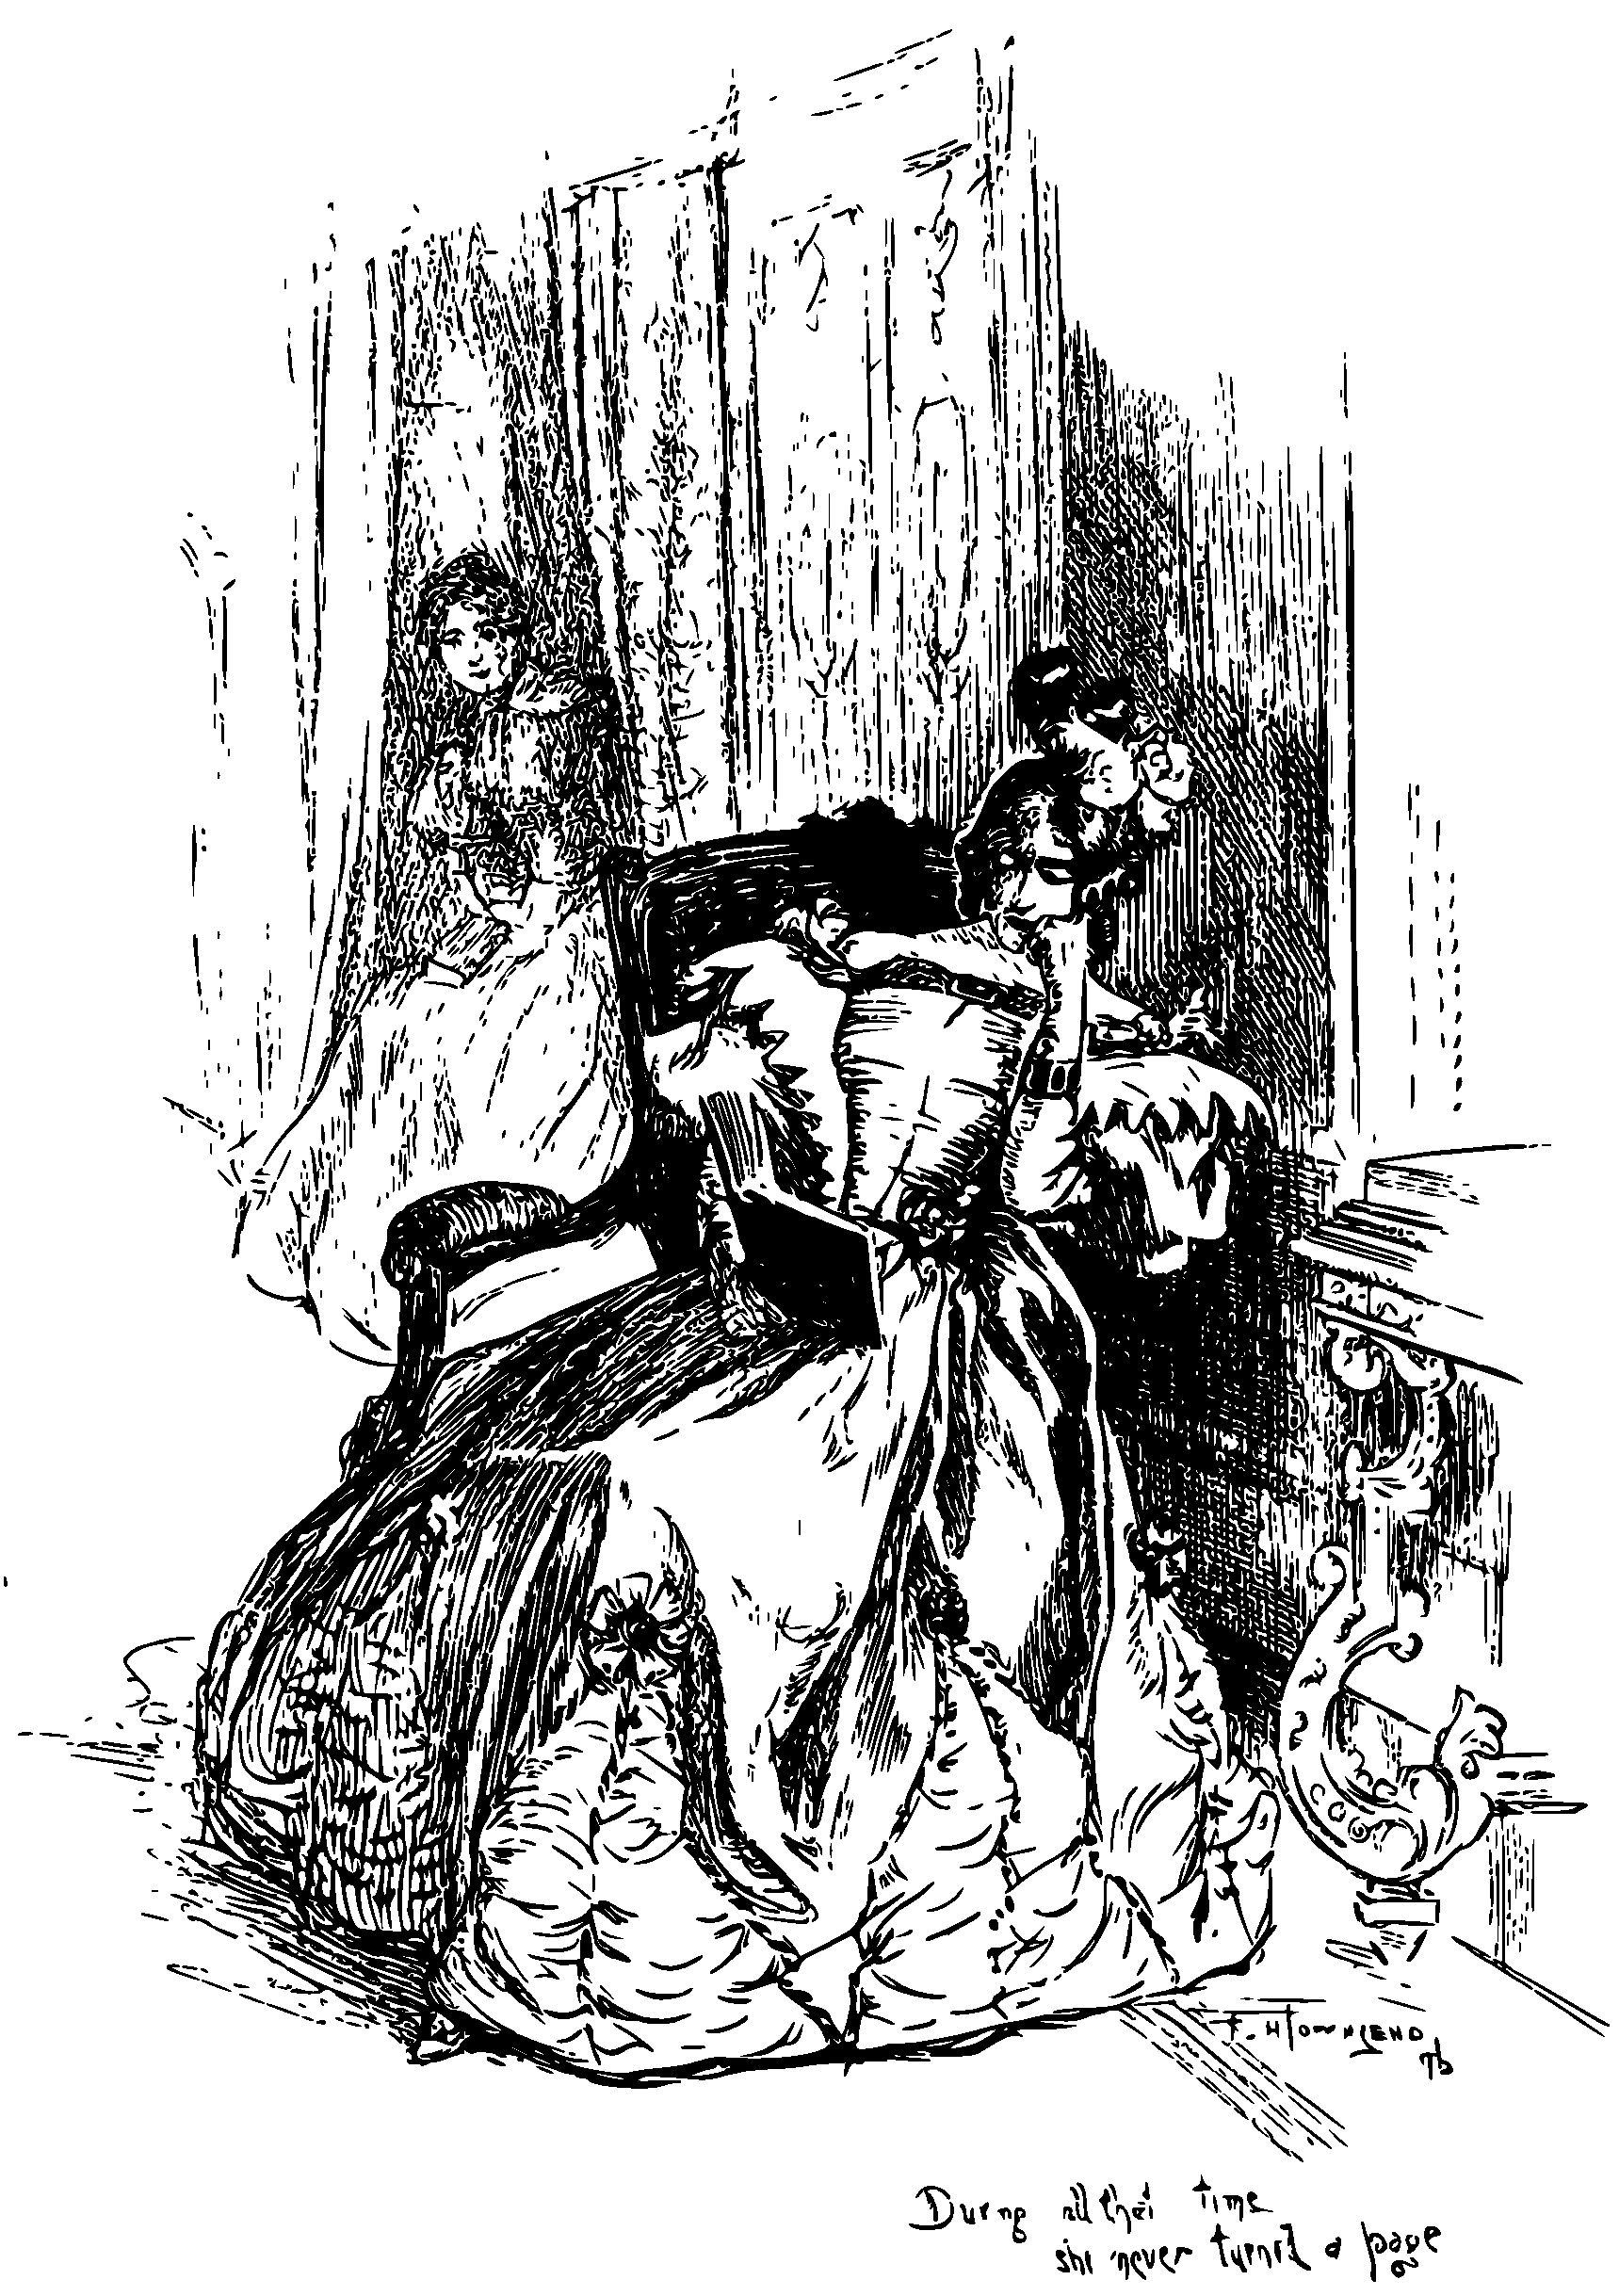
\includegraphics[width=\linewidth]{images/p184b.pdf}
	\end{sidecaption}
\end{figure}

Meantime, Mary Ingram, Amy and Louisa Eshton, declared they dared not go
alone; and yet they all wished to go. A negotiation was opened through
the medium of the ambassador, Sam; and after much pacing to and fro,
till, I think, the said Sam's calves must have ached with the exercise,
permission was at last, with great difficulty, extorted from the
rigorous Sibyl, for the three to wait upon her in a body.

Their visit was not so still as Miss Ingram's had been: we heard
hysterical giggling and little shrieks proceeding from the library; and
at the end of about twenty minutes they burst the door open, and came
running across the hall, as if they were half-scared out of their wits.

\enquote{I am sure she is something not right!} they cried, one and
all. \enquote{She told us such things! She knows all about us!} and
they sank breathless into the various seats the gentlemen hastened to
bring them.

Pressed for further explanation, they declared she had told them of
things they had said and done when they were mere children; described
books and ornaments they had in their boudoirs at home: keepsakes that
different relations had presented to them. They affirmed that she had
even divined their thoughts, and had whispered in the ear of each the
name of the person she liked best in the world, and informed them of
what they most wished for.

Here the gentlemen interposed with earnest petitions to be further
enlightened on these two last-named points; but they got only blushes,
ejaculations, tremors, and titters, in return for their importunity.
The matrons, meantime, offered vinaigrettes and wielded fans; and again
and again reiterated the expression of their concern that their warning
had not been taken in time; and the elder gentlemen laughed, and the
younger urged their services on the agitated fair ones.

In the midst of the tumult, and while my eyes and ears were fully
engaged in the scene before me, I heard a hem close at my elbow: I
turned, and saw Sam.

\enquote{If you please, miss, the gipsy declares that there is another
	young single lady in the room who has not been to her yet, and she
	swears she will not go till she has seen all. I thought it must be you:
	there is no one else for it. What shall I tell her?}

\enquote{Oh, I will go by all means,} I answered: and I was glad of the
unexpected opportunity to gratify my much-excited curiosity. I slipped
out of the room, unobserved by any eye---for the company were gathered
in one mass about the trembling trio just returned---and I closed the
door quietly behind me.

\enquote{If you like, miss,} said Sam, \enquote{I'll wait in the hall
	for you; and if she frightens you, just call and I'll come in.}

\enquote{No, Sam, return to the kitchen: I am not in the least afraid.}
Nor was I; but I was a good deal interested and excited.
